
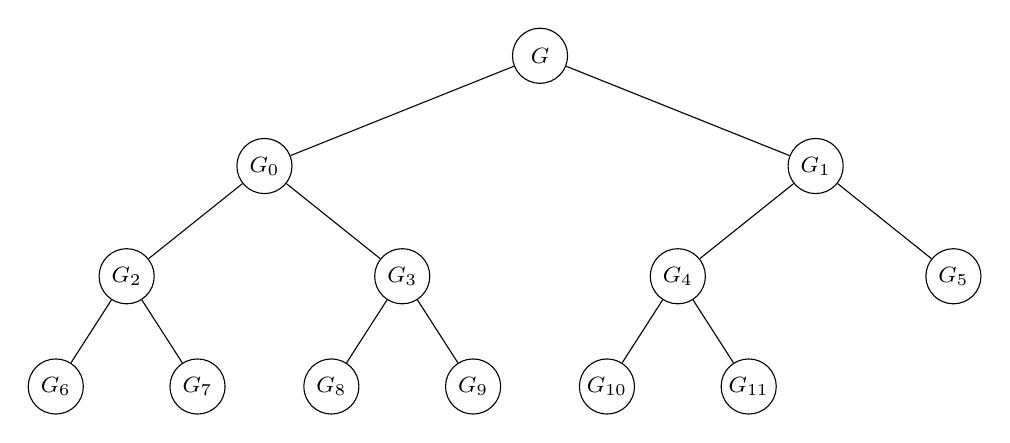
\begin{tikzpicture}[
	level distance=1.4cm,
	every node/.style={circle, draw, minimum size=7mm, inner sep=1pt, font=\footnotesize},
	edge from parent/.style={draw, -},
	level 1/.style={sibling distance=7cm},
	level 2/.style={sibling distance=3.5cm},
	level 3/.style={sibling distance=1.8cm},
	]
	
	\node {$G$}
	child {node {$G_0$}
		child {node {$G_{2}$}
			child {node {$G_6$}}
			child {node {$G_7$}}
		}
		child {node {$G_{3}$}
			child {node {$G_8$}}
			child {node {$G_9$}}
		}
	}
	child {node {$G_1$}
		child {node {$G_{4}$}
			child {node {$G_{10}$}}
			child {node {$G_{11}$}}
		}
		child {node {$G_{5}$}}
	};
	
\end{tikzpicture}
